\section*{23.04 \quad Радиационное затухание}

\begin{itemize}
	\item $\vec{F}_{\text{рад}} = -\eta \vec{v} = -\eta \dot{\vec{r}}$
	
	$m\ddot{\vec{r}} = -\eta \dot{\vec{r}} \underbrace{- k\vec{r}}_{\substack{\text{квазиупругая сила} \\ \text{(возвращ. оболочку обратно)}}}$
	\item $\ddot{\vec{r}} + \frac{\eta}{m} \dot{\vec{r}} + \frac{k}{m} \vec{r} = 0$
	
	$\ddot{\vec{r}} + 2\beta \dot{\vec{r}} + \omega_0^2 \vec{r} = 0$
	
	$\vec{r}(t) = \vec{r}_0 \cdot \exp{i\alpha t}$
	
	$\alpha^2 + 2\beta\alpha + \omega_0^2 = 0$
\end{itemize}

\begin{figure}[H]
	\centering
	\begin{tikzpicture}
		\draw[thick] (0,0) circle (1);
		\filldraw (0,0) circle (1.5pt);
		\draw[->, thick] (0,0) -- (0.5, 0.5) node[right] {$\vec{r}$};
		
		\node[right] at (2, 0.5) {$\vec{r}(t) = \vec{r}_0 \cdot \exp{-\beta t} \cdot \exp{i\omega t}$};
		\node[right] at (2, -0.2) {$\vec{p}(t) = q\vec{r}(t) = \underbrace{\vec{p}_0 \cdot e^{-\beta t} e^{i\omega t}}_{\text{осциллирующий дипольный момент}}$};
		
		\node[right, align=left] at (8, 0.5) {
			$\alpha_{1,2} = -\beta \pm \sqrt{\beta^2 - \omega_0^2} = -\beta \pm i\omega_0 \sqrt{1 - \frac{\beta^2}{\omega_0^2}} = $ \\
			$ = -\beta \pm i\omega_0 \qty(1 - \frac{1}{2}\frac{\beta^2}{\omega_0^2}) \approx -\beta \pm i\omega_0$
		};
		\node[right] at (8, -0.5) {$\omega_0 \sim 10^{16} \si{\per\second} \qquad \beta \sim 10^8 \si{\per\second}$};
	\end{tikzpicture}
\end{figure}

\begin{equation}
	E = E_0 \cdot \exp{-\beta t} \cdot \exp{i\omega_0 t} \qquad 
	\begin{aligned}
		& t \ge 0 \\
		& E = 0 \text{ при } t < 0
	\end{aligned}
\end{equation}

\begin{figure}[H]
	\centering
	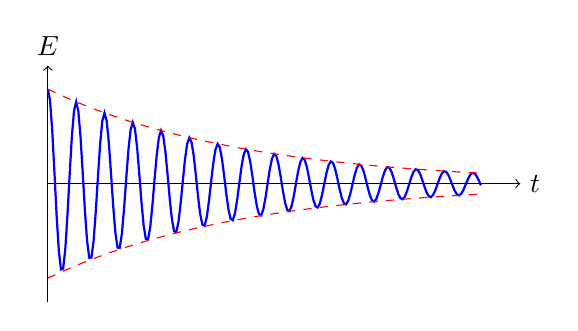
\begin{tikzpicture}
		\draw[->] (0, -1.5) -- (0, 1.5) node[above] {$E$};
		\draw[->] (0, 0) -- (6, 0) node[right] {$t$};
		
		\draw[thick, blue, samples=200, domain=0:5.5] plot (\x, {1.2 * exp(-0.4*\x) * cos(\x * 1000)});
		\draw[dashed, red, samples=50, domain=0:5.5] plot (\x, {1.2 * exp(-0.4*\x)});
		\draw[dashed, red, samples=50, domain=0:5.5] plot (\x, {-1.2 * exp(-0.4*\x)});
	\end{tikzpicture}
\end{figure}

\begin{itemize}
	\item $E = \frac{1}{4\pi\varepsilon_0} \frac{\ddot{p}}{c^2 R} \cdot \sin\theta$
	
	$E = \frac{1}{4\pi\varepsilon_0} \cdot \frac{-\omega_0^2 p_0 e^{-\beta t} \sin\theta}{c^2 R} e^{i\omega_0 t}$
	
	\item $I = \frac{1}{c\mu_0} E E^* = \frac{1}{16\pi^2\varepsilon_0} \cdot \frac{\omega_0^4 \cdot p_0^2 \cdot e^{-2\beta t} \sin^2\theta}{R^2 c^3}$
	
	$\frac{1}{c} = \sqrt{\mu_0 \varepsilon_0}$
\end{itemize}

$\ddot{\vec{p}} = (i\omega_0 - \beta)^2 p_0 e^{-\beta t} e^{i\omega_0 t} = (-\omega_0^2 - 2i\beta\omega_0 + \beta^2) p_0 e^{-\beta t} e^{i\omega_0 t} \approx -\omega_0^2 p_0 e^{-\beta t} e^{i\omega_0 t}$

\begin{figure}[H]
	\centering
	\begin{tikzpicture}
		\draw[->] (0, -0.5) -- (0, 2) node[right] {$I$};
		\draw[->] (0, 0) -- (4, 0) node[right] {$t$};
		\draw[thick, blue, samples=100, domain=0:3.5] plot (\x, {1.5 * exp(-1.5*\x)});
		
		\draw[dashed] (0.66, 0) -- (0.66, 0.55);
		\node[below] at (0.66, 0) {$\tau \sim 10^{-8} \si{\second}$};
	\end{tikzpicture}
\end{figure}
\vspace{-1.5cm}
\begin{align*}
	& \beta = \frac{1}{\tau} \\
	& \colorbox{green!20}{$I = I_0 \cdot e^{-\frac{t}{\tau}} e^{i\omega_0 t}$} \text{ --- опечатка в конспекте, интенсивность не комплексная} \\
	& \text{Должно быть: } \colorbox{green!20}{$I = I_0 \cdot e^{-2\beta t} = I_0 \cdot e^{-t/\tau_{ \text{рад} }}$} \text{, где } \tau_{ \text{рад} } = \frac{1}{2\beta}.
\end{align*}


\section*{Спектр излучения атома Томсона. Однородное уширение спектральной линии}

$E(t) = \Re \underbrace{E_0 e^{-\beta t} e^{i\omega_0 t}} = E_0 e^{-\beta t} \underbrace{\cos\omega_0 t}_{\frac{\exp{i\omega_0 t} + \exp{-i\omega_0 t}}{2}}$

$E(\omega) = \frac{1}{2\pi} \int\limits_0^\infty E(t) \cdot e^{-i\omega t} dt = \frac{E_0}{4\pi} \int\limits_0^\infty \qty[ e^{[-\beta + i(\omega_0 - \omega)]t} + e^{[-\beta - i(\omega + \omega_0)]t} ] dt = \frac{E_0}{4\pi} \cdot \frac{1}{\beta + i(\omega - \omega_0)} + \frac{E_0}{4\pi} \cdot \frac{1}{\beta + i(\omega + \omega_0)}$

$I \sim E E^* = I_0 \frac{1}{\beta^2 + (\omega - \omega_0)^2} + \underbrace{I_0 \frac{1}{\beta^2 + (\omega + \omega_0)^2}}_{\substack{\text{пренебрегаем, т.к.} \\ -\omega_0 \text{ не имеет физ. смысла}}}$

\begin{figure}[H]
	\centering
	\begin{tikzpicture}
		% Временной график
		\begin{scope}[shift={(0,0)}]
			\draw[->] (0, -1) -- (0, 1) node[above] {$E$};
			\draw[->] (0, 0) -- (3, 0) node[right] {$t$};
			\draw[thick, blue, samples=100, domain=0:2.5] plot (\x, {0.8 * exp(-0.8*\x) * cos(\x * 1000)});
			\node[below] at (1.5, -1) {$I(\omega) - ?$};
		\end{scope}
		
		% Спектральный график
		\begin{scope}[shift={(6,0)}]
			\draw[->] (-3, 0) -- (3, 0) node[right] {$\omega$};
			\draw[->] (0, 0) -- (0, 2) node[above] {$I(\omega)$};
			
			\draw[thick, blue, samples=100, domain=0:2.5] plot (\x, {1.5 / (1 + 10*(\x-1.2)^2)});
			\draw[dashed, blue, samples=100, domain=-2.5:0] plot (\x, {1.5 / (1 + 10*(\x+1.2)^2)});
			
			\draw[dashed] (1.2, 0) -- (1.2, 1.5);
			\node[below] at (1.2, 0) {$\omega_0$};
			\draw[<->] (0.88, 0.75) -- (1.52, 0.75);
			\node[above] at (1.2, 0.75) {$2\beta$};
			\node[below] at (0.88, 0) {$\omega_0-\beta$};
			\node[below] at (1.6, 0) {$\omega_0+\beta$};
			
			\node[below] at (-1.2, 0) {$-\omega_0$};
			
			\draw[->] (1.5, 1.2) -- (2, 1.5) node[right] {Лоренцовский контур};
		\end{scope}
	\end{tikzpicture}
\end{figure}

\begin{itemize}
	\item \textbf{Ширина на полувысоте:}
	
	$\frac{I_0}{2} = I_0 \cdot \frac{1}{\beta^2 + (\omega - \omega_0)^2} \implies \Delta\omega = 2\beta$
	
	$\Delta\omega = \omega - \omega_0 = \pm \beta$
	
	$\omega = \omega_0 \pm \beta$
	
	$\tau_{\text{уд}} \ll \tau_{\text{изл}} = \frac{1}{\beta}$
	
	Однородное естественное уширение
\end{itemize}

\section*{Столкновительное уширение}

Высокая плотность, $\tau_{\text{уд}} \ll \tau_{\text{рад}}$, пренебрегаем $\beta$.

\begin{figure}[H]
	\centering
	\begin{tikzpicture}
		% Огибающая цугов
		\begin{scope}[shift={(0,0)}]
			\draw[->] (0, -1) -- (0, 1.5) node[above] {$E$};
			\draw[->] (0, 0) -- (3, 0) node[right] {$t$};
			\draw[dashed] (0, 1) to[out=-20, in=170] (2.5, 0.2);
			\draw[dashed] (0, -1) to[out=20, in=190] (2.5, -0.2);
			\draw[thick, blue] (0,0) sin (0.2, 0.9) cos (0.4, 0) sin (0.6, -0.8) cos (0.8, 0) sin (1, 0.7) cos (1.2, 0) sin (1.4, -0.5);
			
			\draw[dashed] (0.8, -1) -- (0.8, 1);
			\node[below] at (0.8, -1) {$\tau_{\text{уд}}$};
			\node[below] at (1.5, -1.5) {конечный цуг};
		\end{scope}
		
		% Спектр одного цуга
		\begin{scope}[shift={(5, 0)}]
			\draw[->] (-2, 0) -- (2, 0);
			\draw[->] (0, 0) -- (0, 1.5);
			\draw[thick, blue, samples=100, domain=-1.8:1.8] plot (\x, {1.2 * (sin(\x*150)/(\x*150))^2});
			
			\node[align=left] at (2.5, 1) {для одного цуга};
			\draw[->] (1.5, 1) -- (0.5, 0.5);
		\end{scope}
		
		% Форма цуга
		\begin{scope}[shift={(10, 0)}]
			\draw[->] (-1.5, 0) -- (1.5, 0) node[right] {$t$};
			\draw[->] (0, 0) -- (0, 1.5) node[above] {$E$};
			\draw[thick, blue] (-1, 0) -- (-1, 0.8) -- (1, 0.8) -- (1, 0);
			\node[below] at (-1, 0) {$-\frac{\tau}{2}$};
			\node[below] at (1, 0) {$\frac{\tau}{2}$};
		\end{scope}
	\end{tikzpicture}
\end{figure}

$E(t) = E_0 \cdot e^{i\omega_0 t}, \quad -\frac{\tau}{2} \le t \le \frac{\tau}{2}$

$I(\omega) = I_0 \qty[ \int\limits_{-\tau/2}^{\tau/2} E(t) e^{-i\omega t} dt ]^2 = I_0 \cdot \frac{\sin^2\qty((\omega - \omega_0)\frac{\tau}{2})}{\qty[(\omega - \omega_0)\frac{\tau}{2}]^2} \cdot \frac{\tau^2}{4}$

$\underbrace{P(t)}_{\substack{\text{вероятность, что} \\ \text{столкновения} \\ \text{не будет}}} = \frac{1}{\langle \tau_{\text{уд}} \rangle} \cdot e^{-\frac{t}{\langle \tau_{\text{уд}} \rangle}}$

$I(\omega) = \int\limits_0^\infty I(\omega, t) P(t) dt = I_0 \int\limits_0^\infty \frac{\sin^2\qty((\omega - \omega_0)\frac{t}{2})}{(\omega - \omega_0)^2} \frac{1}{\tau_{\text{уд}}} \cdot e^{-\frac{t}{\tau_{\text{уд}}}} dt =$

$= \frac{I_0}{(\omega - \omega_0)^2} \frac{1}{\tau_{\text{уд}}} \int\limits_0^\infty \qty(1 - \cos\Delta\omega t) e^{-\frac{t}{\tau_{\text{уд}}}} dt = \frac{I_0}{\Delta\omega^2 \tau_{\text{уд}}} \qty[ \tau_{\text{уд}} - \frac{\tau_{\text{уд}}}{(\Delta\omega)^2 + \qty(\frac{1}{\tau_{\text{уд}}})^2} ] =$

\begin{equation}
	= I_0 \cdot \frac{1}{(\omega - \omega_0)^2 + \qty(\frac{1}{\tau_{\text{уд}}})^2} \quad \text{--- это Лоренцовский контур.}
\end{equation}
добавляется это: $\Delta\omega \sim 2\qty(\frac{1}{\tau_{\text{уд}}})$

\section*{Доплеровское уширение}

$\omega = \omega_0\qty(1 \pm \frac{v_x}{c})$ -- эффект Доплера

$v_x = \frac{c(\omega - \omega_0)}{\omega_0} \qquad dv_x = \frac{c}{\omega_0} d\omega$

$\frac{dn}{n} = f(v_x) = \qty(\frac{m}{2\pi kT})^{1/2} e^{-\frac{m v_x^2}{2kT}} dv_x$ \quad $v_x \in (v_x, v_x + dv_x)$
$\omega \in (\omega_0, \omega_0 + d\omega)$

$\frac{dn}{n} = f(\omega) = \frac{c}{\omega_0} \qty(\frac{m}{2\pi kT})^{1/2} e^{-\frac{m c^2}{2kT} \frac{(\omega - \omega_0)^2}{\omega_0^2}} d\omega$

$I(\omega) \sim f(\omega)$

\begin{equation}
	\colorbox{orange!30}{$I(\omega) = I_0 \cdot \exp{ - \frac{mc^2}{2kT} \frac{(\omega - \omega_0)^2}{\omega_0^2} }$ \quad --- Доплеровский контур}
\end{equation}

\begin{figure}[H]
	\centering
	\begin{tikzpicture}
		\draw[->] (-3, 0) -- (3, 0) node[right] {$\omega$};
		\draw[->] (0, 0) -- (0, 3) node[above] {$I(\omega)$};
		
		\draw[thick, blue, samples=100, domain=-2.5:2.5] plot (\x, {2.5 * exp(-1.5*\x*\x)});
		\draw[dashed, red, samples=100, domain=-2.8:2.8] plot (\x, {2.5 / (1 + 2*\x*\x)});
		
		\node[below] at (0, 0) {$\omega_0$};
		\node[above] at (0, 2.5) {$I_0$};
		
		\node[right, blue, align=left] at (1.5, 2) {гауссовский / доплеровский \\ контур};
		\node[right, red] at (1.5, 1) {лоренцовский контур};
		\node[left, blue] at (-0.5, 1.5) {$D$};
		\node[left, red] at (-1, 0.8) {$L$};
	\end{tikzpicture}
\end{figure}

Фойгт (Voight profile): $V(\omega) = \int\limits_0^\infty D(\omega') L(\omega - \omega') d\omega'$ -- т.е. \textbf{свертка}
$\hookrightarrow$ учитываем и Доплера, и Лоренца

$L = I_0 \frac{1}{\beta^2 + (\omega - \omega_0)^2} \qquad D = I_0 e^{-\frac{mc^2}{2kT} \frac{(\omega - \omega_0)^2}{\omega_0^2}}$

\section*{Нормальный эффект Зеемана}

$\hookrightarrow$ Зееман и Лоренц получили Нобелевскую премию

\begin{figure}[H]
	\centering
	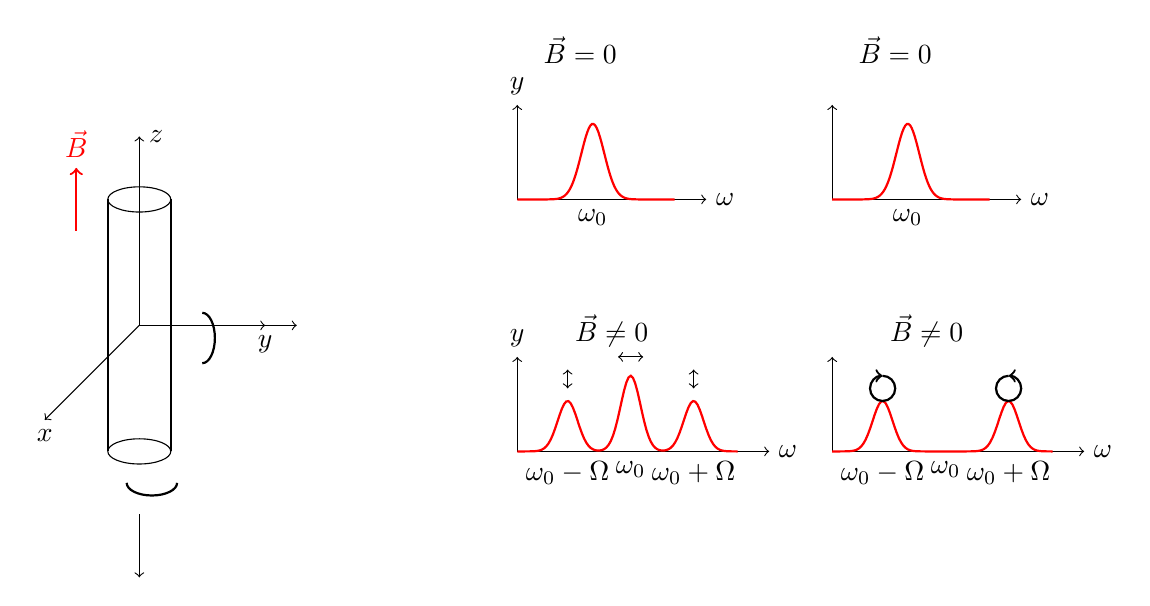
\begin{tikzpicture}[scale=0.8]
		% Цилиндр с B
		\begin{scope}[shift={(0,0)}]
			\draw[thick] (-0.5, -2) -- (-0.5, 2);
			\draw[thick] (0.5, -2) -- (0.5, 2);
			\draw (0, 2) ellipse (0.5 and 0.2);
			\draw (0, -2) ellipse (0.5 and 0.2);
			\draw[->, thick, red] (-1, 1.5) -- (-1, 2.5) node[above] {$\vec{B}$};
			
			\draw[->] (0, 0) -- (0, 3) node[right] {$z$};
			\draw[->] (0, 0) -- (2, 0) node[below] {$y$};
			\draw[->] (0, 0) -- (-1.5, -1.5) node[below] {$x$};
			
			\draw[thick] (1, 0.2) arc (90:-90:0.2 and 0.4);
			\draw[->] (1.5, 0) -- (2.5, 0);
			
			\draw[thick] (-0.2, -2.5) arc (180:360:0.4 and 0.2);
			\draw[->] (0, -3) -- (0, -4);
		\end{scope}
		
		% Спектры
		\begin{scope}[shift={(6, 2)}]
			\node[above] at (1, 2) {$\vec{B} = 0$};
			\draw[->] (0, 0) -- (3, 0) node[right] {$\omega$};
			\draw[->] (0, 0) -- (0, 1.5) node[above] {$y$};
			\draw[thick, red, samples=100, domain=0:2.5] plot (\x, {1.2*exp(-15*(\x-1.2)*(\x-1.2))});
			\node[below] at (1.2, 0) {$\omega_0$};
		\end{scope}
		
		\begin{scope}[shift={(11, 2)}]
			\node[above] at (1, 2) {$\vec{B} = 0$};
			\draw[->] (0, 0) -- (3, 0) node[right] {$\omega$};
			\draw[->] (0, 0) -- (0, 1.5);
			\draw[thick, red, samples=100, domain=0:2.5] plot (\x, {1.2*exp(-15*(\x-1.2)*(\x-1.2))});
			\node[below] at (1.2, 0) {$\omega_0$};
		\end{scope}
		
		\begin{scope}[shift={(6, -2)}]
			\node[above] at (1.5, 1.5) {$\vec{B} \neq 0$};
			\draw[->] (0, 0) -- (4, 0) node[right] {$\omega$};
			\draw[->] (0, 0) -- (0, 1.5) node[above] {$y$};
			\draw[thick, red, samples=100, domain=0:3.5] plot (\x, {0.8*exp(-20*(\x-0.8)*(\x-0.8)) + 1.2*exp(-20*(\x-1.8)*(\x-1.8)) + 0.8*exp(-20*(\x-2.8)*(\x-2.8))});
			\node[below] at (0.8, 0) {$\omega_0-\Omega$};
			\node[below] at (1.8, 0) {$\omega_0$};
			\node[below] at (2.8, 0) {$\omega_0+\Omega$};
			
			\draw[<->] (0.8, 1) -- (0.8, 1.3);
			\draw[<->] (1.6, 1.5) -- (2.0, 1.5);
			\draw[<->] (2.8, 1) -- (2.8, 1.3);
		\end{scope}
		
		\begin{scope}[shift={(11, -2)}]
			\node[above] at (1.5, 1.5) {$\vec{B} \neq 0$};
			\draw[->] (0, 0) -- (4, 0) node[right] {$\omega$};
			\draw[->] (0, 0) -- (0, 1.5);
			\draw[thick, red, samples=100, domain=0:3.5] plot (\x, {0.8*exp(-20*(\x-0.8)*(\x-0.8)) + 0.8*exp(-20*(\x-2.8)*(\x-2.8))});
			\node[below] at (0.8, 0) {$\omega_0-\Omega$};
			\node[below] at (1.8, 0) {$\omega_0$};
			\node[below] at (2.8, 0) {$\omega_0+\Omega$};
			
			\draw[->, thick] (0.8, 1.2) arc (90:-270:0.2);
			\draw[<-, thick] (2.8, 1.2) arc (90:-270:0.2);
		\end{scope}
	\end{tikzpicture}
\end{figure}

\begin{itemize}
	\item $\vec{B} = 0 \qquad m\ddot{\vec{r}} = -\eta\dot{\vec{r}} - k\vec{r} \implies \ddot{\vec{r}} + 2\beta\dot{\vec{r}} + \omega_0^2\vec{r} = 0$
	
	$\vec{p} = q\vec{r} = p_x\vec{e}_x + p_y\vec{e}_y + p_z\vec{e}_z \qquad \vec{r} = x\vec{e}_x + y\vec{e}_y + z\vec{e}_z$
	
	\begin{equation*}
		\begin{cases}
			\ddot{x} + 2\beta\dot{x} + \omega_0^2 x = 0 \\
			\ddot{y} + 2\beta\dot{y} + \omega_0^2 y = 0 \\
			\ddot{z} + 2\beta\dot{z} + \omega_0^2 z = 0
		\end{cases}
	\end{equation*}
	
	\item $\vec{B} \neq 0 \qquad m\ddot{\vec{r}} = -\eta\dot{\vec{r}} - k\vec{r} + q[\dot{\vec{r}}, \vec{B}]$
	
	$\ddot{\vec{r}} + 2\beta\dot{\vec{r}} + \omega_0^2\vec{r} - \frac{q}{m}[\dot{\vec{r}}, \vec{B}] = 0$
	
	$\ddot{\vec{r}} + 2\beta\dot{\vec{r}} + \omega_0^2\vec{r} - 2[\dot{\vec{r}}, \vec{\Omega}] = 0$
	
	\colorbox{orange!30}{$\vec{\Omega} = \frac{qB}{2m} \vec{e}_z \text{ --- Ларморовская частота}$}
\end{itemize}

$[\dot{\vec{r}}, \vec{\Omega}] = [(\dot{x}\vec{e}_x + \dot{y}\vec{e}_y + \dot{z}\vec{e}_z), \Omega\vec{e}_z] = \Omega\qty( \dot{x}\underbrace{[\vec{e}_x, \vec{e}_z]}_{-\vec{e}_y} + \dot{y}\underbrace{[\vec{e}_y, \vec{e}_z]}_{\vec{e}_x} + \dot{z}\underbrace{[\vec{e}_z, \vec{e}_z]}_{0} ) = -\Omega\dot{x}\vec{e}_y + \Omega\dot{y}\vec{e}_x$

$\ddot{\vec{r}} = \ddot{x}\vec{e}_x + \ddot{y}\vec{e}_y + \ddot{z}\vec{e}_z$

\begin{equation}
	\begin{cases}
		\ddot{x} + 2\beta\dot{x} + \omega_0^2 x - 2\Omega\dot{y} = 0 \\
		\ddot{y} + 2\beta\dot{y} + \omega_0^2 y + 2\Omega\dot{x} = 0 \\
		\ddot{z} + 2\beta\dot{z} + \omega_0^2 z = 0
	\end{cases}
\end{equation}

\begin{itemize}
	\item Перейдем от базиса $(\vec{e}_x, \vec{e}_y, \vec{e}_z)$ к $(\vec{e}_+, \vec{e}_-, \vec{e}_z)$: \quad $\vec{e}_+ = \frac{\vec{e}_x + i\vec{e}_y}{\sqrt{2}}, \quad \vec{e}_- = \frac{\vec{e}_x - i\vec{e}_y}{\sqrt{2}}$.
	
	\item $\vec{r} = r_+\vec{e}_+ + r_-\vec{e}_- + z\vec{e}_z$
	
	$[\dot{\vec{r}}, \vec{\Omega}] = [ (\dot{r}_+\vec{e}_+ + \dot{r}_-\vec{e}_- + \dot{z}\vec{e}_z), \Omega\vec{e}_z ] = \dot{r}_+ \Omega \underbrace{[\vec{e}_+, \vec{e}_z]}_{\dots} + \dot{r}_- \Omega \underbrace{[\vec{e}_-, \vec{e}_z]}_{\dots} = \dot{r}_+ \Omega \qty[ \frac{\vec{e}_x + i\vec{e}_y}{\sqrt{2}}, \vec{e}_z ] + \dot{r}_- \Omega \qty[ \frac{\vec{e}_x - i\vec{e}_y}{\sqrt{2}}, \vec{e}_z ] = $
	
	$ = \frac{\dot{r}_+ \Omega}{\sqrt{2}} (-\vec{e}_y + i\vec{e}_x) + \frac{\dot{r}_- \Omega}{\sqrt{2}} (-\vec{e}_y - i\vec{e}_x) = i \dot{r}_+ \Omega \frac{\vec{e}_x + i\vec{e}_y}{\sqrt{2}} - i \dot{r}_- \Omega \frac{\vec{e}_x - i\vec{e}_y}{\sqrt{2}} = i \dot{r}_+ \Omega \vec{e}_+ - i \dot{r}_- \Omega \vec{e}_-$
\end{itemize}

\begin{equation*}
	\begin{cases}
		\ddot{r}_+ + 2\beta\dot{r}_+ + \omega_0^2 r_+ - 2i\Omega\dot{r}_+ = 0 \quad (1) \\
		\ddot{r}_- + 2\beta\dot{r}_- + \omega_0^2 r_- + 2i\Omega\dot{r}_- = 0 \quad (2) \\
		\ddot{z} + 2\beta\dot{z} + \omega_0^2 z = 0
	\end{cases}
\end{equation*}

(1) $\to$ ищем решение $r_+ = C_+ e^{\alpha t}$
\begin{align*}
	& \alpha_+^2 + 2\beta\alpha_+ - 2i\Omega\alpha_+ + \omega_0^2 = 0 \\
	& \alpha_+^2 + 2\alpha_+(\beta - i\Omega) + \omega_0^2 = 0 \\
	& \alpha_+ = -\beta + i\Omega \pm \sqrt{(\beta - i\Omega)^2 - \omega_0^2} \approx -\beta + i\Omega \pm i\omega_0 \quad (\text{т.к. } \omega_0 \gg \beta) \quad \text{*выбираем } +i\omega_0 \\
	& \alpha_+ \approx -\beta + i(\Omega + \omega_0)
\end{align*}

(2) $\to$ по аналогии $\alpha_- \approx -\beta - i\Omega \pm i\omega_0$.

\begin{equation}
	\begin{cases}
		\vec{r}_+ = \vec{e}_+ C_+ e^{-\beta t} e^{i(\omega_0 + \Omega)t} \\
		\vec{r}_- = \vec{e}_- C_- e^{-\beta t} e^{i(\omega_0 - \Omega)t} \\
		\vec{r}_z = \vec{e}_z z = \vec{e}_z C_z e^{-\beta t} e^{i\omega_0 t}
	\end{cases}
\end{equation}

$\vec{p}_+ = q\vec{r}_+, \quad \vec{p}_- = q\vec{r}_-, \quad \vec{p}_z = q\vec{r}_z$

\begin{nb}
	Эта теория работает только для атомов, у которых спин равен 0.
\end{nb}

\section*{Взаимодействие света с веществом}

\begin{itemize}
	\item Будем учитывать рассеяние и поглощение.
	\item Рассматриваем немагнитные и непроводящие среды ($\mu=1, j=0$).
	\item Группа (ансамбль) атомов Томсона: $\vec{P} = \frac{\sum \vec{p}_i}{V} ; \vec{P} = n \vec{p}$.
\end{itemize}

Среда:
\begin{itemize}
	\item линейная ($\vec{P} \sim \vec{E}$: связь между ними линейная)
	\item нелинейная ($\chi = \chi(\vec{E})$ -- т.е. $\chi$ зависит от $\vec{E}$)
	\item однородная ($\chi = \text{const}$)
	\item неоднородная ($\chi = \chi(\vec{r})$)
	\item изотропная (св-ва во всех направлениях одинаковы: $\vec{P} \uparrow\uparrow \vec{E}$)
	\item анизотропная ($\vec{P} \not\parallel \vec{E}$)
\end{itemize}

$\vec{D} = \varepsilon_0 \vec{E} + \vec{P}$ \\
$\vec{P} = \varepsilon_0 \chi \vec{E}$ \\
$\chi = \hat{\chi}$ (тензор), $P_i = \sum \chi_{ij} E_j$ *в разреженных средах $\chi = N\alpha$ \\
$\vec{D} = \varepsilon_0 \vec{E} + \varepsilon_0 \chi \vec{E} = \varepsilon_0 \varepsilon \vec{E}$ \\
$\varepsilon = 1 + \chi$

\subsection*{(1) Динамическая поляризуемость атома Томсона}

\begin{figure}[H]
	\centering
	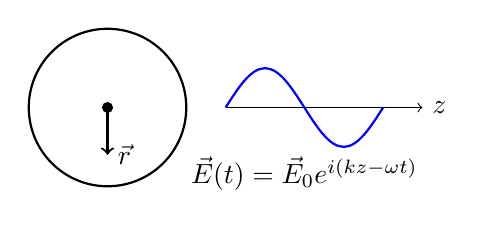
\begin{tikzpicture}
		\draw[thick] (0,0) circle (1);
		\fill (0,0) circle (2pt);
		\draw[->, thick] (0,0) -- (0, -0.6) node[right] {$\vec{r}$};
		
		\draw[->] (1.5, 0) -- (4, 0) node[right] {$z$};
		\draw[thick, blue] (1.5, 0) sin (2, 0.5) cos (2.5, 0) sin (3, -0.5) cos (3.5, 0);
		\node[below] at (2.5, -0.5) {$\vec{E}(t) = \vec{E}_0 e^{i(kz - \omega t)}$};
	\end{tikzpicture}
\end{figure}

II закон Ньютона: $m\ddot{\vec{r}} = -\eta\dot{\vec{r}} - k\vec{r} + q\vec{E} \quad \big| : m \quad \vec{F}_{\text{внеш.}}$

$\ddot{\vec{r}} + 2\beta\dot{\vec{r}} + \omega_0^2\vec{r} = \frac{q}{m}\vec{E}$

$\ddot{\vec{r}} + 2\beta\dot{\vec{r}} + \omega_0^2\vec{r} = \frac{q}{m}\vec{E}_0 e^{i(kz - \omega t)}$

\begin{itemize}
	\item В разреженных средах $\chi(\omega) = N\alpha(\omega)$
	
	$\varepsilon(\omega) = 1 + \chi(\omega)$
	
	$\vec{D} = \varepsilon_0 \vec{E} + \vec{P} = \varepsilon_0 \vec{E} + \varepsilon_0 N\alpha \vec{E}$
	
	$\vec{P} = \varepsilon_0 \chi \vec{E}$
\end{itemize}

\begin{equation}
	\varepsilon(\omega) = 1 + \frac{N q^2}{m\varepsilon_0} \cdot \frac{1}{\omega_0^2 - \omega^2 - 2i\beta\omega} = \varepsilon'(\omega) + i\varepsilon''(\omega)
\end{equation}
$n(\omega) = \sqrt{\varepsilon(\omega)} = n'(\omega) + i n''(\omega)$

Решение дифура: $\vec{p} + 2\beta\dot{\vec{p}} + \omega_0^2\vec{p} = \frac{q^2}{m}\vec{E}_0 e^{i(kz - \omega t)}$

$\vec{p} = \vec{p}_{\text{общ}}(t) + \vec{p}_{\text{част}}(t)$

$\vec{p}_{\text{общ}}(t)$ затухает за $10^{-8} \si{\second}$ ($\vec{p}_{\text{общ}}(t) = p_0 e^{-\beta t} e^{i\omega_0 t}$)

$\vec{p}_{\text{част}} \equiv \vec{p} = \vec{p}_0 e^{i(kz - \omega t)}$

$(-\omega^2 - 2\beta i\omega + \omega_0^2) \vec{p}_0 = \frac{q^2}{m} \vec{E}_0$

$\vec{p}_0 = \frac{q^2}{m} \frac{1}{\omega_0^2 - \omega^2 - 2i\beta\omega} \vec{E}_0$

$\vec{p} = \frac{q^2}{m} \frac{1}{\omega_0^2 - \omega^2 - 2i\beta\omega} \vec{E} \implies \vec{p} = \alpha(\omega) \vec{E}$

\begin{nb}
	$\alpha(\omega) = \frac{q^2}{m} \frac{1}{\omega_0^2 - \omega^2 - 2\beta i\omega}$ --- динамическая поляризуемость атома Томсона
	
	$\alpha(\omega) = \alpha'(\omega) + i\alpha''(\omega)$
\end{nb}